% MeanFlowPrecond network (meanflow_precond.py): a SongUNet that predicts the
% average velocity u_theta(z_r, r, t, c). The state z_r is concatenated with the
% 10-channel condition c_t; the state time r enters the noise/positional
% embedding (scaled by time_scale), and the interval length (t-r) enters as
% fixed sin/cos Fourier features through the augment_labels pathway. Both are
% merged into the timestep conditioning that is broadcast to every residual block.
\documentclass[border=12pt]{standalone}
% Shared style for the MeanFlow thesis figures.
% Clean academic grayscale, in the spirit of the nntikz examples
% (rounded gray!10 blocks, -latex arrows). Self-contained: this does NOT
% depend on the legacy presentation/meanflow_workflow/src/mf_style.tex.
\usepackage{amsmath,amssymb,bm}
\usepackage{tikz}
\usetikzlibrary{positioning,arrows.meta,calc,fit,backgrounds,shapes.geometric,chains,decorations.pathmorphing}

\tikzset{
  % --- generic nodes ---------------------------------------------------
  base/.style    ={rounded corners=2.5pt, draw, line width=0.8pt, align=center,
                   inner sep=5pt, font=\small, text=black!88},
  block/.style   ={base, fill=gray!10},
  data/.style    ={base, fill=white},                       % data / tensors
  net/.style     ={base, fill=gray!22, line width=1.0pt},   % trained network
  frozen/.style  ={base, fill=gray!4, draw=black!60,        % frozen network
                   dash pattern=on 3pt off 2pt},
  loss/.style    ={base, fill=gray!10, line width=1.0pt,    % loss / scalar
                   double, double distance=1.2pt},
  emph/.style    ={base, fill=gray!10, line width=1.3pt},   % highlighted box
  % --- operator glyphs -------------------------------------------------
  op/.style      ={circle, draw, line width=0.8pt, fill=white,
                   minimum size=4.6mm, inner sep=0, font=\footnotesize},
  concat/.style  ={rectangle, rounded corners=1pt, draw, fill=black!72,
                   text=white, font=\scriptsize\bfseries, inner sep=2.5pt},
  % --- arrows ----------------------------------------------------------
  arrow/.style   ={-{Latex[length=2.4mm]}, line width=0.8pt, draw=black!82},
  arrowc/.style  ={arrow, rounded corners=3pt},
  thinarrow/.style={-{Latex[length=2.0mm]}, line width=0.6pt, draw=black!55},
  loopback/.style={-{Latex[length=2.4mm]}, line width=0.8pt, draw=black!55,
                   dashed, dash pattern=on 4pt off 3pt},
  % --- containers / annotation ----------------------------------------
  group/.style   ={rounded corners=5pt, draw=black!40, line width=0.7pt,
                   dashed, dash pattern=on 3pt off 2.5pt, fill=black!2,
                   inner sep=8pt},
  ttl/.style     ={font=\bfseries\large, text=black!88},
  sub/.style     ={font=\itshape\footnotesize, text=black!55},
  lab/.style     ={font=\scriptsize, text=black!70},
  tag/.style     ={font=\scriptsize\bfseries, text=black!60},
  % small sine glyph used to mark Fourier / positional embeddings
  sinewave/.style={decorate, decoration={snake, amplitude=0.6mm,
                   segment length=2.2mm}},
}

% legend swatch helper: \swatch{<style>}{<label>}
\newcommand{\swatch}[2]{%
  \tikz[baseline=-0.5ex]\node[#1, minimum width=3.6mm, minimum height=2.8mm,
    inner sep=0]{};\;#2}

\begin{document}
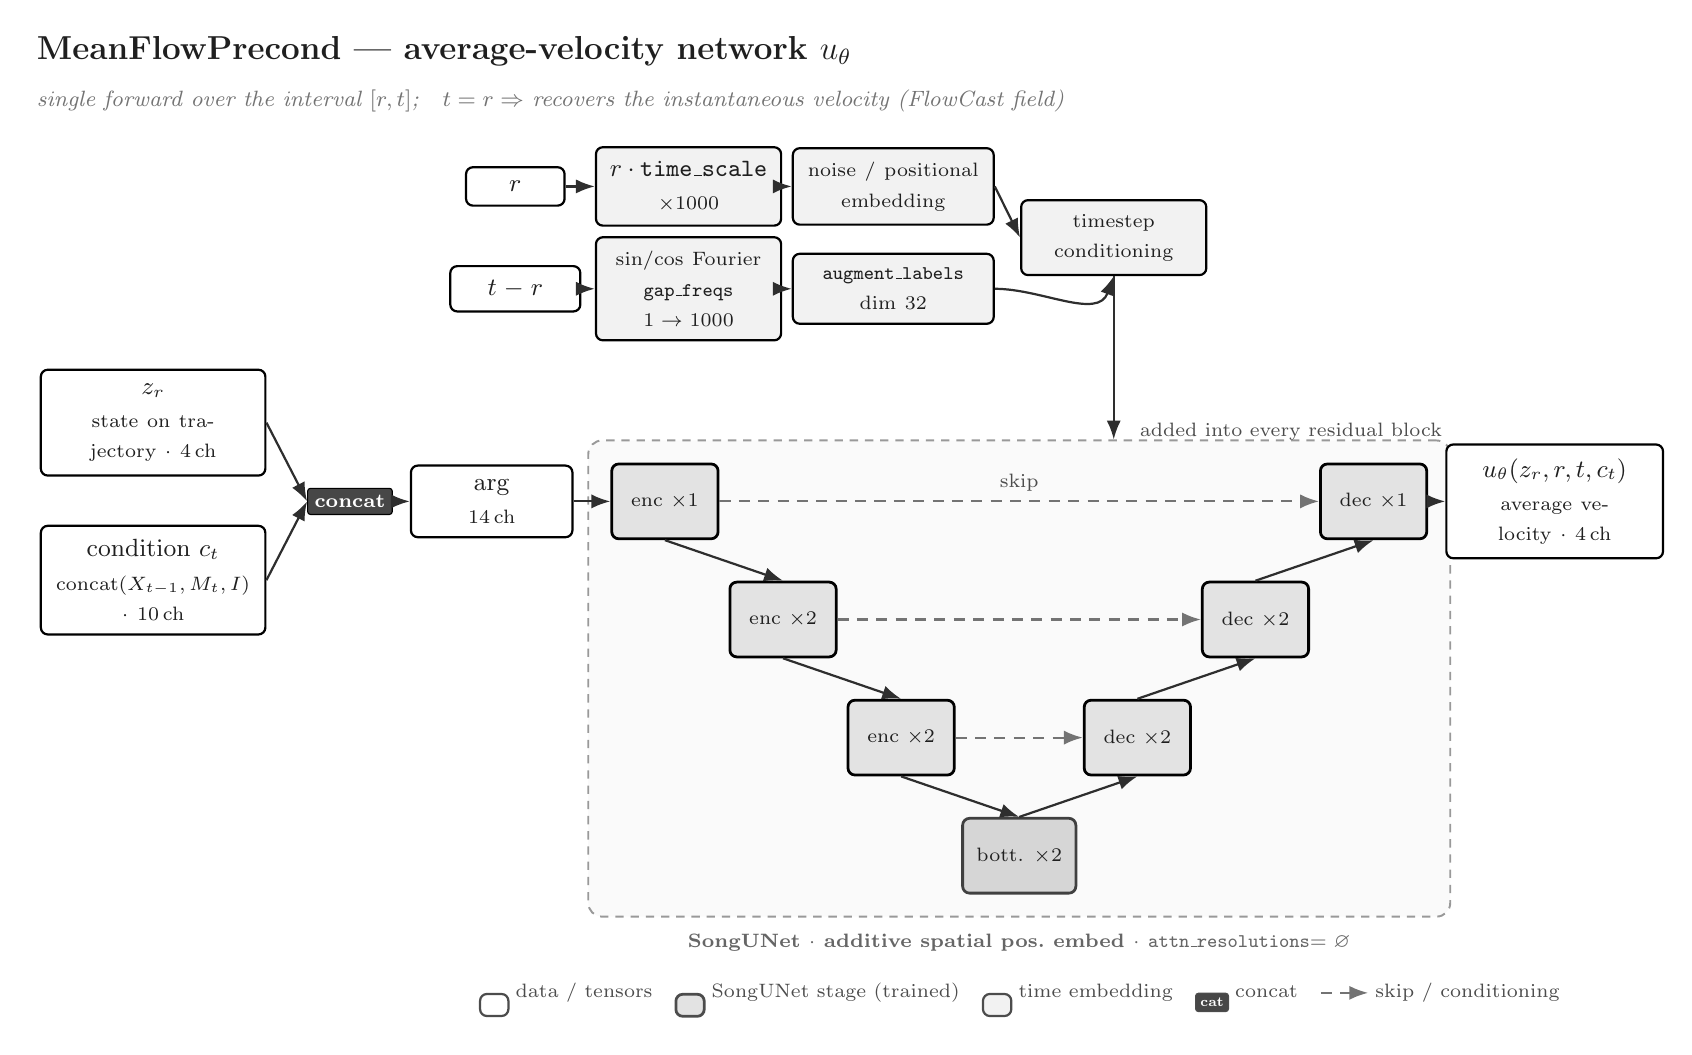
\begin{tikzpicture}[node distance=9mm]

  % ============================ inputs + concat ============================
  \node[data, text width=2.5cm] (zr) at (0,1.0)
    {$z_r$\\[1pt]\scriptsize state on trajectory $\cdot$ 4\,ch};
  \node[data, text width=2.5cm] (ct) at (0,-1.0)
    {condition $c_t$\\[1pt]\scriptsize $\mathrm{concat}(X_{t-1},M_t,I)$ $\cdot$ 10\,ch};
  \node[concat] (cc) at (2.5,0) {concat};
  \node[data, text width=1.7cm] (arg) at (4.3,0)
    {$\mathrm{arg}$\\[1pt]\scriptsize 14\,ch};

  % ============================ SongUNet (clean symmetric U) ============================
  % encoder steps down-right, bottleneck at the bottom, decoder steps up-right.
  % channel_mult = [1,2,2,2,2]; levels share heights so skips are exact horizontals.
  \tikzset{ustage/.style={net, minimum height=0.95cm, minimum width=1.35cm, font=\scriptsize}}
  \node[ustage] (e1) at (6.5, 0.0)  {enc $\times1$};
  \node[ustage] (e2) at (8.0,-1.5)  {enc $\times2$};
  \node[ustage] (e3) at (9.5,-3.0)  {enc $\times2$};
  \node[ustage, draw=black!75, fill=gray!32] (bk) at (11.0,-4.5) {bott. $\times2$};
  \node[ustage] (d3) at (12.5,-3.0) {dec $\times2$};
  \node[ustage] (d2) at (14.0,-1.5) {dec $\times2$};
  \node[ustage] (d1) at (15.5, 0.0) {dec $\times1$};

  \begin{scope}[on background layer]
    \node[group, fit=(e1)(bk)(d1), inner sep=8pt] (unet) {};
  \end{scope}
  \node[tag, anchor=north] at ($(unet.south)+(0,-0.8mm)$)
    {SongUNet $\cdot$ additive spatial pos.\ embed $\cdot$ \texttt{attn\_resolutions}$=\varnothing$};

  % ============================ output ============================
  \node[data, text width=2.4cm] (out) at (17.8, 0.0)
    {$u_\theta(z_r,r,t,c_t)$\\[1pt]\scriptsize average velocity $\cdot$ 4\,ch};

  % ============================ main data path (the U) ============================
  \draw[arrow] (zr.east) -- (cc.west);
  \draw[arrow] (ct.east) -- (cc.west);
  \draw[arrow] (cc.east) -- (arg.west);
  \draw[arrow] (arg.east) -- (e1.west);
  \draw[arrow] (e1.south) -- (e2.north);
  \draw[arrow] (e2.south) -- (e3.north);
  \draw[arrow] (e3.south) -- (bk.north);
  \draw[arrow] (bk.north)  -- (d3.south);
  \draw[arrow] (d3.north) -- (d2.south);
  \draw[arrow] (d2.north) -- (d1.south);
  \draw[arrow] (d1.east) -- (out.west);

  % ============================ skip connections (exact horizontals) ============================
  \draw[loopback] (e1.east) -- node[lab,above,pos=0.5]{skip} (d1.west);
  \draw[loopback] (e2.east) -- (d2.west);
  \draw[loopback] (e3.east) -- (d3.west);

  % ============================ time-embedding rails -> single injection ============================
  % rail 1: r -> x time_scale -> noise/positional embedding
  \node[data, text width=0.9cm] (r) at (4.6,4.0) {$r$};
  \node[block, text width=2.0cm] (rsc) at (6.8,4.0)
    {$r\cdot\texttt{time\_scale}$\\[1pt]\scriptsize $\times 1000$};
  \node[block, text width=2.2cm] (remb) at (9.4,4.0)
    {\scriptsize noise / positional\\embedding};
  % rail 2: (t - r) -> sin/cos Fourier -> augment_labels
  \node[data, text width=1.3cm] (gap) at (4.6,2.7) {$t-r$};
  \node[block, text width=2.0cm] (four) at (6.8,2.7)
    {\scriptsize sin/cos Fourier\\\texttt{gap\_freqs} $1\!\to\!1000$};
  \node[block, text width=2.2cm] (aug) at (9.4,2.7)
    {\scriptsize \texttt{augment\_labels}\\dim $32$};
  % merge into a single timestep-conditioning bundle
  \node[block, text width=2.0cm] (emb) at (12.2,3.35)
    {\scriptsize timestep\\conditioning};

  \draw[arrow] (r.east)   -- (rsc.west);
  \draw[arrow] (rsc.east) -- (remb.west);
  \draw[arrow] (gap.east)  -- (four.west);
  \draw[arrow] (four.east) -- (aug.west);
  \draw[arrow] (remb.east) -- (emb.west);
  \draw[arrow] (aug.east)  to[out=0,in=-110] (emb.south);
  % one clean arrow into the network top (stops above all skips); broadcast note
  \draw[arrow] (emb.south) -- (emb.south |- unet.north)
        node[lab, anchor=west, pos=0.95, xshift=2mm]{added into every residual block};

  % ============================ title + subtitle ============================
  \node[ttl, anchor=south west] (title) at (-1.6,5.4)
    {MeanFlowPrecond --- average-velocity network $u_\theta$};
  \node[sub, anchor=north west] at ($(title.south west)+(0,-0.5mm)$)
    {single forward over the interval $[r,t]$; \; $t=r \Rightarrow$ recovers the instantaneous velocity (FlowCast field)};

  % ============================ legend ============================
  \node[lab, anchor=north] at ($(unet.south)+(0,-7mm)$)
    {\swatch{data}{data / tensors}\quad
     \swatch{net}{SongUNet stage (trained)}\quad
     \swatch{block}{time embedding}\quad
     \tikz[baseline=-0.5ex]\node[concat, scale=0.7]{cat};\;concat\quad
     \tikz[baseline=-0.5ex]\draw[loopback](0,0)--(0.6,0);\;skip / conditioning};

\end{tikzpicture}
\end{document}
